%\documentclass{article}
%\usepackage{graphicx,subfigure}
%\begin{document}

\begin{figure}[!h]
  \centering
  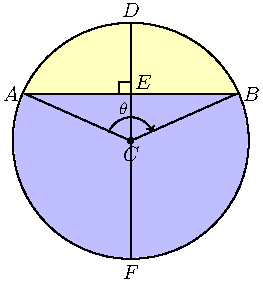
\includegraphics[width=0.7\textwidth]{xsect.pdf}
  \caption{Circle representing a fibre cross-section segmented by a chord AB into para and ortho cortex segments. The para cortex is the yellow segment above chord AB, the orthocortex is the blue segment below chord AB. The parameter $m = D_{p}/D_{o}$ is defined as a ratio of the distance DE to the distance EF. The angle ACB subtended by the chord is referred to as $\theta$ in the text.}
  \label{fig:opmeas}
\end{figure}

%\end{document}

